\section{Data-Driven Modeling, Control and Tools for Cyber-Physical Energy Systems}

In 2013, a report by the U.S. National Climate Assessment provided evidence that the most recent decade was the nation's warmest on record~\cite{melillo2014climate} and 2015 is very likely to become the hottest year on record since the beginning of weather recording in 1880~\cite{noaa}. 
Heat waves in summer and polar vortexes in winter are growing longer and pose increasing challenges to an already over-stressed electric grid. 

Furthermore, with the increasing penetration of renewable generation, the electricity grid is also experiencing a shift from predictable and dispatchable electricity generation to variable and non-dispatchable generation. 
This adds another level of uncertainty and volatility to the electricity grid as the relative proportion of variable generation vs. traditional dispatchable generation increases.
%The organized electricity markets across the world all use some variant of real-time price for wholesale electricity. 
%The real-time electricity market at PJM, one of the world's largest independent system operator (ISO), is a spot market where electricity prices are calculated at five-minute intervals based on the grid operating conditions. 
The volatility due to the mismatch between electricity generation and supply further leads to volatility in the wholesale price of electricity.
For \eg the polar vortex triggered extreme weather events in the U.S. in January 2014, which caused many electricity customers to experience increased costs.
Parts of the Pennsylvania-New Jersey-Maryland (PJM) electricity grid experienced a $86$ fold increase in the price of electricity from $\$31/\si{\mega\watt\hour}$ to $\$2,680/\si{\mega\watt\hour}$ in a matter of a few minutes~\cite{volatility}. 
Similarly, the summer price spiked $32$ fold from an average of $\$25/\si{\mega\watt\hour}$ to $\$800/\si{\mega\watt\hour}$ in July of 2015.
%Such events show how unforeseen and uncontrollable circumstances can greatly affect electricity prices that impact ISOs, suppliers, and customers. 
Energy industry experts are now considering the concept that extreme weather, more renewables and resulting electricity price volatility, could become the new norm.

\begin{figure}[t]
\centering
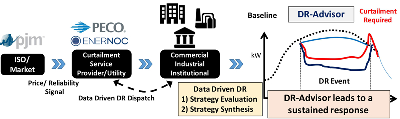
\includegraphics[width=0.9\columnwidth]{figs/demandresponse}
\caption{Majority of DR today is manual and rule-based. The fixed rule based DR is inconsistent and could under-perform compared to the required curtailment, resulting in DR penalties. Using data-driven models DR-Advisor uses DR strategy evaluation and DR strategy synthesis for a sustained and sufficient curtailment.}
\label{fig:demand_response}
\vspace{-10pt}
\end{figure}

Across the United States, electric utilities and independent service operators (ISOs or grid coordinators) are devoting increasing attention and resources to demand response (DR)~\cite{goldman2010coordination}. It is considered as a reliable means of mitigating the uncertainty and volatility of renewable generation and extreme weather conditions and improving the grid's efficiency and reliability.
The potential demand response resource contribution from all U.S. demand response programs is estimated to be nearly 72,000 megawatts (MW), or about 9.2 percent of U.S. peak demand~\cite{federal2008assessment} making DR the largest virtual generator in the U.S. national grid.
The annual revenue to end-users from DR markets with PJM ISO alone is more than $\$700$ million~\cite{pjm}. 
Global DR revenue is expected to reach nearly $\$40$ billion from 2014 through 2023~\cite{navigant}.


%The volatility in real-time electricity prices poses the biggest operational and financial risk for large scale end-users of electricity such as large commercial buildings, industries and institutions~\cite{Mulhall2014327}; often referred to as \textit{C/I/I} consumers. 
In order to shield themselves from the volatility and risk of high prices, such consumers must be more flexible in their electricity demand. 
Consequently, large commercial, industrial and institutional customers are increasingly looking to demand response programs to help manage their electricity costs.
As shown in \figref{demand_response}, DR programs involve a voluntary response of a building to a price signal or a load curtailment request from the utility or the curtailment service provider. 
Upon successfully meeting the required curtailment level the end-users are financially rewarded, but may also incur penalties for under-performing and not meeting a required level of load curtailment.


\subsection{Challenges}

On the surface demand response may seem simple. Reduce your power when asked to and get paid. 
However, in practice, one of the biggest challenges with end-user demand response for large scale consumers of electricity is the following: \emph{Upon receiving the notification for a DR event, what actions must the end-user take in order to achieve an adequate and a sustained DR curtailment?} 
This is a hard question to answer because of the following reasons:\vspace{4pt}

\textbf{1. Modeling complexity and heterogeneity:}
~Unlike the automobile or the aircraft industry, each building is designed and used in a different way and therefore, it must be uniquely modeled. 
%Learning predictive models of building's dynamics using first principles based approaches (\eg with EnergyPlus~\cite{Crawley2001319}) is very cost and time prohibitive and requires retrofitting the building with several sensors~\cite{sturzeneggermodel};
The user expertise, time, and associated sensor costs required to develop a model of a single building (\eg with EnergyPlus~\cite{Crawley2001319}) is very high~\cite{sturzeneggermodel} - often taking 5-12 months to model and tune the model.
This is because usually a building modeling domain expert requires the geometry of a building from the building design and equipment layout plans, detailed information about material properties, and of  equipment and operational schedules. \vspace{4pt}
%There is always a gap between the modeled and the real building and the domain expert must then manually tune the model to match the measured data from the building~\cite{new2012autotune}. 
%\item \textbf{Limitations of rule-based DR}: The building's operating conditions, internal thermal disturbances and environmental conditions must all be taken into account to make appropriate DR control decisions, which is not possible with using rule-based and pre-determined DR strategies since they do not account for the state of the building but are instead based on best practices and rules of thumb. The performance of a rule-based DR strategy is inconsistent and can lead to reduced amount of curtailment which could result in penalties to the end-user. In our work, we show how a data-driven DR algorithm outperforms a rule-based strategy by $17\%$ while accounting for thermal comfort.
%Rule based DR strategies have the advantage of being simple but they do not account for the state of the building and weather conditions during a DR event.
%Despite this lack of predictability, rule-based DR strategies account for the majority of DR approaches.

\textbf{2. Control complexity and scalability:}
~Upon receiving a notification for a DR event, the building's facilities manager must determine an appropriate DR strategy to achieve the required load curtailment. 
These control strategies can include adjusting zone temperature set-points, supply air temperature and chilled water temperature set-point, dimming or turning off lights, decreasing duct static pressure set-points and restricting the supply fan operation \etc 
For a large building, it is difficult to asses the effect of one control action on other sub-systems and on the building's overall power consumption because the building sub-systems are tightly coupled. 
%Consider the case of the University of Pennsylvania's campus, which has over a hundred different buildings and centralized chiller plants. In order to perform campus wide DR, the facilities manager must account for several hundred thousand set-points and their impact on the different buildings. 
Therefore, it is extremely difficult for a human operator to accurately gauge the building's or a campus's response.\vspace{4pt}

\textbf{3. Interpretability of modeling and control:}
~Predictive models for buildings, regardless how sophisticated, lose their effectiveness unless they can be interpreted by human experts and facilities managers in the field.
For \eg artificial neural networks (ANN) obscure physical control knobs and interactions and hence, are difficult to interpret by building facilities managers.
Therefore, the required solution must be transparent, human centric and highly interpretable.

%The goal with data-driven methods for cyber-physical energy systems is to make the best of both worlds; i.e. simplicity of rule based approaches and the predictive capability of model based strategies, but without the expense of first principle or grey-box model development.

\subsection{Real-Time Data-driven Demand Response}

We have developed a method called DR-Advisor (Demand Response-Advisor)~\cite{dr_advisor}, which acts as a recommender system for the building's facilities manager and provides the power consumption prediction and control actions for meeting the required load curtailment and maximizing the economic reward.  
Using historical meter and weather data along with set-point and schedule information, DR-Advisor builds a family of interpretable regression trees to learn non-parametric data-driven models for predicting the power consumption of the building (Figure~\ref{fig:overview}).
DR-Advisor can be used for real-time demand response baseline prediction, strategy evaluation and, most importantly, for control synthesis, without having to learn first principles based models of the building:\vspace{4pt}

\textbf{1. DR Baseline Prediction:} A baseline is an estimate of the electricity that would have been consumed by a customer in the absence of a demand response event. Typical demand response programs rely upon financial incentive for customers based on the extent to which they reduce their energy consumption and therefore require a reliable system to measure the energy reduction. For this reason the measurement and verification of demand response is the most critical component of any DR program. Using regression trees based approaches, DR-Advisor achieves a prediction accuracy of $93\%$ to $98.9\%$ for baseline estimates of eight buildings on the Penn campus by just analyzing data as shown in Figure~\ref{fig:overview}.\vspace{4pt}
\begin{figure}[t]
\centering
\includegraphics[width=0.85\columnwidth]{figs/overview.pdf}
\vspace{-3pt}
\caption{DR-Advisor Architecture for real-time demand response}
\label{fig:overview}
\vspace{-16pt}
\end{figure}

\textbf{2. DR Strategy Evaluation:} A DR strategy refers to what sequence of control actions, and at what times, a system (lighting, HVAC or plug loads) will actuate. 
Furthermore, there could be several of such fixed DR strategies, but only one specific strategy can be used at a time. 
This brings us to our question, \emph{how can we choose good DR strategies from a pre-determined set of strategies ?}
Instead of predicting the baseline power consumption $\hat{Y_{base}}$, in this case we want the ability to predict the actual response of the building $\hat{Y_{kW}}$ due to any given strategy.
 At the beginning of the DR event we use the auto-regressive tree for predicting the response of the building due to each rule-based strategy and choose the one which performs the best over the predicted horizon. The prediction and strategy evaluation is re-computed periodically throughout the event.\vspace{4pt}

%%%%%%%%%%%%%%%%%%%%%%%%%%%%%%%%%%%%%%%%%%%%%%%%%%%%%%
\begin{figure*}
%\vspace{-10pt}
	\begin{center}
%	\subfigure [Wired Network Control System] {
%	\includegraphics[width=0.25\textwidth]{figs/NCS_ppt.pdf} 
%	\label{fig:ncs_wired}
%	}
	\subfigure [Wired Network Control] {
			\includegraphics[width=0.24\textwidth]{figs/wired_system.pdf}
			\label{fig:System_wired}
		}	
	\subfigure [Wireless Network Controlled System] {
			\includegraphics[width=0.37\textwidth]{figs/wcns_conv.pdf}
			\label{fig:wncs}
		}	
	\subfigure [Wireless Control Network] {
			\includegraphics[width=0.28\textwidth]{figs/wcn_system.pdf}
			\label{fig:wcn}
		}	
	\end{center}	
\vspace{-10pt}
\label{fig:ncs_full}
\caption{Standard architectures for Networked Control Systems; (a) Wired system with a shared bus and dedicated controller; (b) Red links/nodes - routing data from the plant's sensors to the controller; Blue links/nodes - routing data from the controller to the plant's actuators; (c) A multi-hop wireless control network used as a distributed controller.}
%\vspace{-5pt}
\end{figure*}
%%%%%%%%%%%%%%%%%%%%%%%%%%%%%%%%%%%%%%%%%%%%%%%%%%%%%%
\textbf{3. DR Control Synthesis:}  While black-box and data-driven machine learning approaches are suitable for prediction, our primary contribution is making them capable of controller synthesis. 
Unlike rule-base DR, which does not account for building state and external factors, in DR synthesis the optimal control actions are derived based on the current state of the building, forecast of outside weather and electricity prices.
We introduce a novel model based control with regression trees (mbCRT) algorithm to enable control with regression trees for real-time DR synthesis. Using the mbCRT algorithm, we can optimally trade off thermal comfort inside the building against the amount of load curtailment. 
While regression trees are a popular choice for prediction based models, this is the first time regression tree based algorithms have been used for controller synthesis with applications in demand response. Our synthesis algorithm outperforms rule based DR strategy by $17\%$ (based on guidelines from Siemens) while maintaining bounds on thermal comfort inside the building.\vspace{4pt}

We have evaluated the performance of DR-Advisor using a mix of real data from 8 buildings (1.2 million square feet) on the campus of the University of Pennsylvania, a large office building in Philadelphia and data-sets from a virtual building test-bed for the Department of Energy's (DoE) large commercial reference building.
We also compared the performance of DR-Advisor against other data-driven methods using a bench-marking data-set from AHRAE's great energy predictor shootout challenge~\cite{kreider1994predicting} and rank second. The first place was achieved by the use of neural networks which are not interpretable, while DR-Advisor with regression trees is highly interpretable by facilities managers and provides them both guidance and provenance for decisions made to control their infrastructure.

